\chapter{Data structures - list boxes and lists}
	\label{ch:data-structures}

	This chapter explains:
	\begin{itemize}
    \item how to use the list box control;
    \item the idea of a list;
    \item how to add, insert and remove items from a list box;
    \item how to obtain the length of a list box;
    \item the idea of an index;
    \item how to carry out typical operations on a list box, such as lookup, addition and searching.
	\end{itemize}


  \section{Introduction}
		A list box control displays a list of string items in a box. It provides a number of facilities, including the ability to select an item in a list by clicking on it, add items and delete items. The list box control is available along with the other controls on the toolbox and can be placed as usual on a form. We will use as an example a shopping list, building it up by adding items one by one. After some items have been added, the list box looks like \Vref{fig:data_listbox_screen}. Each item occupies a single line. If the complete list cannot be displayed in the available space, a scroll bar is automatically displayed. Later we will see how to delete items from the list.
		
		List boxes provide a good introduction to using data structures because they provide a direct, visual representation of the information. This chapter explores using list boxes as data structures and it can be read and studied independently of the chapters on arrays.

		\begin{figure}[bth]
			\centering
			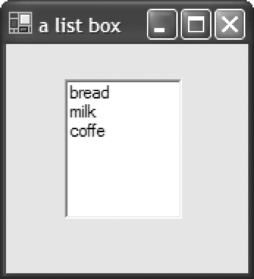
\includegraphics[width=5cm]{data_listbox_screen}
			\caption{A list box.}
			\label{fig:data_listbox_screen}
		\end{figure}

  \section{Lists}
		When we use a list box by dragging it on to the form from the toolbox, we are creating a new instance of the \keyword{ListBox} class. The \keyword{ListBox} class makes use of another class, called a \keyword{List}, to carry out its functions. A list box merely displays information on the form and handles mouse-click events, but a list actually holds the information displayed in a text box. So while a list box supports the events \keyword{Click} and \keyword{DoubleClick} and properties such as \keyword{SelectedItem}, a list provides methods to add and remove items from the list.
		
		For example, if we create a list box named \keyword{Shopping}, then the property \keyword{Shopping.Items} is the list containing the information displayed in the list box:
		\begin{lstlisting}
Dim myList As List
myList = Shopping.Items
		\end{lstlisting}
		We can then use the properties and methods of lists with \keyword{myList}. For example, we can obtain a count of the number of items in the list (and in the list box) as follows:
		\begin{lstlisting}
Dim numberOfItems As Integer
numberOfItems = myList.Count
		\end{lstlisting}
		This series of statements can be written more concisely as follows:
		\begin{lstlisting}
Dim numberOfItems As Integer
numberOfItems = Shopping.Items.Count
		\end{lstlisting}
		in which we have chosen not to explicitly mention the list.


	\section{Adding items to a list}
		The example program shown in \Vref{fig:data_adding_screen} allows the user to add items to a list box. The following method responds to a button-click and places an item of shopping at the end of the list box.
		\begin{figure}[bth]
			\centering
			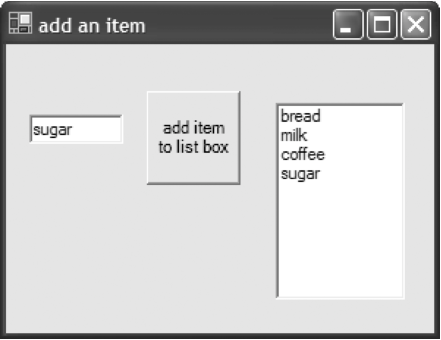
\includegraphics[width=8cm]{data_adding_screen}
			\caption{Adding items to a shopping list.}
			\label{fig:data_adding_screen}
		\end{figure}
		\begin{lstlisting}
Private Sub Button1_Click(sender As System.Object,
		e As System.EventArgs)
		Handles Button1.Click
	Shopping.Items.Add(TextBox1.Text)
End Sub
		\end{lstlisting}
		In this example the name of the list box is \keyword{Shopping}. As we have seen, one of the properties of a list box is \keyword{Items} and this property represents the contents of the list box as an instance of the \keyword{List} class. This class in turn provides a number of methods, one of which is the \keyword{Add} method that allows items to be added to a list. Its parameter is the value to be added to the list. It must be a string.
		
		Another way of placing items in a list box is to do it at design-time. Selecting the \keyword{Items} property of a list box throws up a new window in which items can be inserted into the list box.


	\section{The length of a list}
		Next, here is a method that responds to a button-click and displays a message box containing the number of items currently in the list box.
		\begin{lstlisting}
Private Sub CountButton_Click(sender As System.Object,
		e As System.EventArgs)
		Handles CountButton.Click
	MessageBox.Show(CStr(Shopping.Items.Count))
End Sub
		\end{lstlisting}
		Again we see how the property Items of the list box named \keyword{Shopping} is used. In turn the property \keyword{Count} of the \keyword{List} class is used to obtain the number of items held in the list box.

	\section{Indices}
	A program refers to the items in a list box by an \emph{index}. An index is an integer that says which item is being referred to. The first item has index value 0, the second 1, etc. We can visualize the above list box as a table as shown in \Vref{fig:data_diagram_indices}, with the index values alongside (but not actually stored with the data).
		\begin{figure}[bth]
			\centering
			\begin{tabular}{l|l|}
				\cline{2-2}
				0 & bread\\ \cline{2-2}
				1 & milk\\ \cline{2-2}
				2 & coffee\\ \cline{2-2}
			\end{tabular}
			\caption{Diagram of a list box showing indices.}
			\label{fig:data_diagram_indices}
		\end{figure}
		
		We now look at a program that emphasizes and demonstrates index values. The user clicks on an item in a list box and the program displays the equivalent index value in a text box (\Vref{fig:data_selecting_screen}). When the click event arrives, the following method is called to handle the event.
		\begin{figure}[bth]
			\centering
			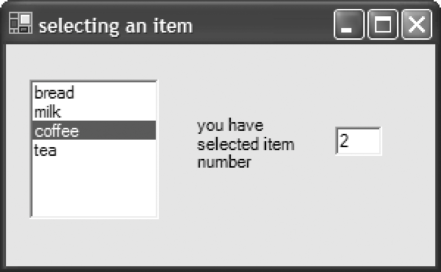
\includegraphics[width=8cm]{data_selecting_screen}
			\caption{Selecting an item from a list box.}
			\label{fig:data_selecting_screen}
		\end{figure}

		\begin{lstlisting}
Private Sub Shopping_Click(
		sender As System.Object,
		e As System.EventArgs)
		Handles Shopping.Click
	TextBox1.Text = CStr(Shopping.SelectedIndex)
End Sub
		\end{lstlisting}
		\keyword{SelectedIndex} is a list box property that provides the index value of the item clicked on (or -1 if nothing has been selected). Running this program emphasizes that the index values are not actually stored as part of a list box, but that the computer knows the values and they can be used as and when necessary. You also confirm, when you run this program, that the index values start at zero (not at 1).

		\begin{stqb}
			\begin{STQ}
				\item In \Vref{fig:data_selecting_screen}, what is the index value of the item bread?
			\end{STQ}
		\end{stqb}
		\Vref{fig:data_displaying_screen} shows a program that allows the user to display the item corresponding to a chosen index value. The code to handle the button-click is:
		\begin{figure}[bth]
			\centering
			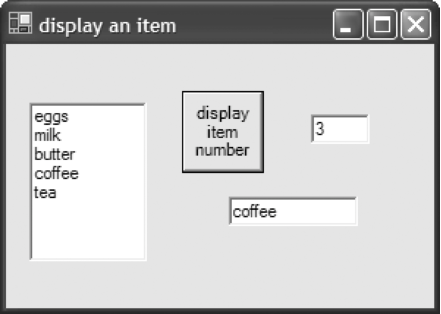
\includegraphics[width=8cm]{data_displaying_screen}
			\caption{Displaying an item from a list box.}
			\label{fig:data_displaying_screen}
		\end{figure}

		\begin{lstlisting}
Private Sub Button1_Click(sender As System.Object,
		e As System.EventArgs)
		Handles Button1.Click
	Dim index As Integer
	index = CInt(IndexTextBox.Text)
	ValueTextBox.Text = CStr(Shopping.Items(index))
End Sub
		\end{lstlisting}
		The program extracts the value from the list box using the expression:
		\begin{lstlisting}
Shopping.Items(index)
		\end{lstlisting}
		In this expression, \keyword{Shopping} is the name of the list box. \keyword{Items} is the property of a list box that gives the contents of the list box, which is a list. Finally the index value is placed in brackets after the name of the list. Thus, for example:
		\begin{lstlisting}
Shopping.Items(2)
		\end{lstlisting}
		would give us the value in the list box at index value 2.
		
		\begin{stqb}
			\begin{STQ}
				\item \Vref{fig:data_displaying_screen}, what item is at index value 1?
			\end{STQ}
		\end{stqb}


	\section{Removing items from a list}
	We have seen how to add items to a list box. Now we consider removing information. The method \keyword{RemoveAt} of the class \keyword{List} removes the item at a particular index value. So if we have a list box \keyword{Shopping}, we can remove the item at index value 3 by:
		\begin{lstlisting}
Shopping.Items.RemoveAt(3)
		\end{lstlisting}
		When this happens, the gap created is closed up.


	\section{Inserting items within a list}
	We have seen how to add items to the end of a list using the method \keyword{Add}. It is also possible to insert items within the body of a list, using method Insert. Given an existing list, we can for example do this:
		\begin{lstlisting}
Shopping.Items.Insert(5, "tea")
		\end{lstlisting}
		The item formerly at index value 5 is moved down the list, along with any subsequent items.
	

	\section{Lookup}
		A table such as a list box is conveniently used for lookup. For example, we can construct a list box (\Vref{fig:data_diagram_lookup}) that contains the names of the months, January to December. Then if someone gives us a month expressed as a number (1 to 12) we can use the table to convert the number to the equivalent text.
		\begin{figure}[bth]
			\centering
			\begin{tabular}{l|l|}
				\cline{2-2}
				0 & January\\ \cline{2-2}
				1 & February\\ \cline{2-2}
				2 & March\\ \cline{2-2}
				3 & etc.\\ \cline{2-2}
			\end{tabular}
			\caption{Diagram of a list box for converting integers to month names.}
			\label{fig:data_diagram_lookup}
		\end{figure}
		
		\Vref{fig:data_conversion_screen} shows how the program looks to its user. We will make this list box invisible (by setting its \keyword{Visible} property to \keyword{False}), since there is no need for the user of the program to know about it.
		\begin{figure}[bth]
			\centering
			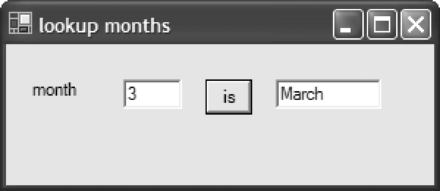
\includegraphics[width=7cm]{data_conversion_screen}
			\caption{The month conversion program.}
			\label{fig:data_conversion_screen}
		\end{figure}

		When the program is designed, we enter the values January, February, March, etc., directly into the \keyword{Items} property of the list box.
		
		When the program runs, a number entered via a text box can be converted as follows:
		\begin{lstlisting}
Private Sub Button1_Click(sender As System.Object,
		e As System.EventArgs)
		Handles Button1.Click
	Dim monthNumber As Integer
	Dim monthName As String
	monthNumber = CInt(MonthNumberTextBox.Text)
	monthName = CStr(Months.Items(monthNumber – 1))
	MonthNameTextBox.Text = monthName
End Sub
		\end{lstlisting}
		The numbers representing a month run from 1 to 12, whereas index values start at 0. Therefore we need to subtract 1 from the month number, as shown, to convert it into an appropriate index. The \keyword{Items} property of a list box allows the program to access the value of an item in the list box named \keyword{Months}.
		
		Using a lookup table as above is an alternative to writing a series of If statements to carry out the conversion, which has the following structure:
		\begin{lstlisting}
If monthNumber = 1 Then
	monthName = "January"
Else
	If monthNumber = 2 Then
		monthName = "February"
	End If
End If
		\end{lstlisting}
		Yet another alternative would be to use a \keyword{Select Case} statement. Employing \keyword{If} statements or a \keyword{Select Case} statement makes use of actions to carry out the conversion. In contrast, using a table (such as a list box) embodies the conversion information more neatly within the table.


	\section{Arithmetic on a list box}
		We now look at a list box, named \keyword{Numbers}, that contains integer numbers and we will carry out arithmetic on the numbers. A list box always contains strings, but one kind of string is a string of digits – a number. \Vref{fig:data_arithmetic_screen} shows a program that allows its user to enter numbers into a list box. Then one button causes the sum of the numbers to be displayed and another button causes the largest number to be displayed.
		\begin{figure}[bth]
			\centering
			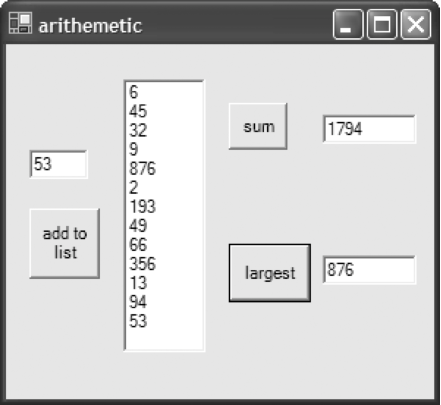
\includegraphics[width=8cm]{data_arithmetic_screen}
			\caption{Arithmetic on a list box.}
			\label{fig:data_arithmetic_screen}
		\end{figure}
		
		Here is the program to add together all the numbers in a list. A \keyword{For} statement is used to run through all the values of the index. Remember index values start at 0. The index of the last item in the list is equal to the length of the list –1. Each value in the list is added to a running total, called \keyword{Sum}, which is initially made equal to 0. Finally the value is placed in a text box.
		\begin{lstlisting}
Private Sub SumButton_Click(sender As System.Object,
			e As System.EventArgs)
			Handles SumButton.Click
	Dim number As Integer
	Dim index As Integer
	Dim sum As Integer
	sum = 0
	For index = 0 To Numbers.Items.Count – 1
		number = CInt(Numbers.Items(index))
		sum = sum + number
	Next 
	SumTextBox.Text = CStr(sum)
End Sub
		\end{lstlisting}
		Next we study a method to find the largest item in a list of numbers. A variable called \keyword{largest} is used to keep track of the largest value. Initially, it is made equal to the value at index 0 in the list box. A For statement is used to process all of the numbers in the list. Each item in the list is compared with \keyword{largest}, and if it is larger, the value of \keyword{largest} is updated.
		\begin{lstlisting}
Private Sub LargestButton_Click(sender As System.Object,
			e As System.EventArgs)
			Handles LargestButton.Click
	Dim number As Integer
	Dim index As Integer
	Dim largest As Integer
	largest = CInt(Numbers.Items(0))
	For index = 1 To Numbers.Items.Count – 1
		number = CInt(Numbers.Items(index))
		If number > largest Then
			largest = number
		End If
	Next 
	LargestTextBox.Text = CStr(largest)
End Sub
		\end{lstlisting}

		\begin{stqb}
			\begin{STQ}
				\item Modify this method very simply so as to find the smallest item in the list.
			\end{STQ}
		\end{stqb}
		These two sections of program illustrate a common feature of programs that manipulate lists: whenever you need to process every item in a list, a \keyword{For} statement is the appropriate tool. Clearly a loop is needed to examine repetitively each item in what might be a long list. The alternative structures for describing a loop are the \keyword{For} statement and the \keyword{While} statement. The \keyword{For} statement is preferable in this case because we know at the outset of the loop how many repetitions are necessary.


	\section{\keyword{For Each}}
		Some \keyword{For} loops can be written more concisely using the \keyword{For Each} statement. For example, the above method to sum up the numbers in a list box can be written:
		\begin{lstlisting}
Private Sub SumButton_Click(sender As System.Object,
			e As System.EventArgs)
			Handles SumButton.Click
	Dim number As Integer
	Dim sum As Integer
	sum = 0
	For Each number As Integer In Numbers.Items
		sum = sum + CInt(number)
	Next
	SumTextBox.Text = CStr(sum)
End Sub
		\end{lstlisting}
		You will see that mention of the index values has vanished. Instead we simply mention the name of a variable (\keyword{number} in this case) that takes on each of the values in the list, one by one.
		
		Although the \keyword{For Each} loop is very concise, it has some disadvantages:
		\begin{enumerate}
			\item	the program cannot use any index values;
			\item	the program cannot change any of the values in the list.
		\end{enumerate}


	\section{Searching}
		This next program carries out a search. It assumes that a list (for example, the shopping list) is already set up and that we want to search the list for some item. The user enters the desired item (for example sugar) into a text box as shown in \Vref{fig:data_searching_screen}.
		\begin{figure}[bth]
			\centering
			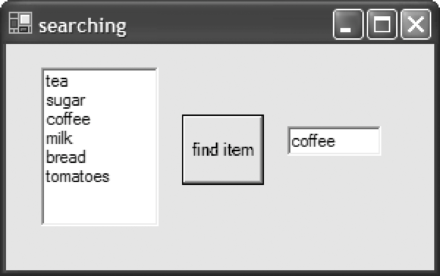
\includegraphics[width=8cm]{data_searching_screen}
			\caption{Searching a list box.}
			\label{fig:data_searching_screen}
		\end{figure}

		The program starts from the first item in the list and continues down the list one item at a time, trying to find the desired item. If it is not found, the index value becomes equal to the size of the list, length, and the loop ends. If the item is found, the \keyword{Boolean} variable found is set to \keyword{True} and the loop terminates. A \keyword{While} statement is used rather than a \keyword{For} statement for controlling the loop, since we do not know in advance how many repetitions will be necessary.
		\begin{lstlisting}
Private Sub Button1_Click(sender As System.Object,
		e As System.EventArgs)
		Handles Button1.Click
	Dim length As Integer
	Dim index As Integer
	Dim found As Boolean
	Dim itemWanted As String
	length = Shopping.Items.Count
	itemWanted = TextBox1.Text
	found = False
	index = 0
	While (found = False) And (index < length)
		If CStr(Shopping.Items(index)) = itemWanted Then
			found = True
			MessageBox.Show("Item found")
		Else
			index = index + 1
		End If
	End While
End Sub
		\end{lstlisting}
		This is a classical serial search method.


	\section{Using a list – generics}
		All the examples we have seen so far use a list box. A list box uses a list to hold the strings. Now we look at using a list directly. The difference is that when you use a list, the contents are not displayed automatically.
		
		Suppose we need to create a list to hold some strings. We do it like this:
		\begin{lstlisting}
Private myList As New List(Of String)
		\end{lstlisting}
		You will see that the name of the class of the objects that the list is to hold is placed in brackets after the keyword Of. This feature goes by the name of generics. It simply means that we can create a list tailored to hold objects of a particular class.
		
		Now that we have created a list to hold strings, we can add some items:
		\begin{lstlisting}
Private Sub AddButton_Click(sender As System.Object,
		e As System.EventArgs)
		Handles Button1.Click
	myList.Add("bread")
	myList.Add("milk")
	myList.Add("coffee")
End Sub
		\end{lstlisting}
		Note that a list automatically expands to accommodate however many items are added. It also contracts when items are removed.
		
		If we need to display the contents of the list, we will need to write code to do it explicitly. We could display the above list in a list box as follows, by copying the string values, one by one:
		\begin{lstlisting}
Private Sub DisplayButton_Click(sender As System.Object,
			e As System.EventArgs)
			Handles Button1.Click
	Dim index As Integer
	For index = 0 To myList.Count - 1
		MyListBox.Items.Add(myList(index))
	Next
End Sub
		\end{lstlisting}
		Notice that the index value is enclosed in brackets after the list name.
		
		This method can be written more concisely using the \keyword{For Each} statement:
		\begin{lstlisting}
Private Sub DisplayButton_Click(sender As System.Object,
			e As System.EventArgs)
			Handles Button1.Click
	For Each s As String In myList
		MyListBox.Items.Add(s)
	Next
End Sub
		\end{lstlisting}

		
	\section{Methods and properties of lists}
		Here are some of the most useful methods and properties that can be used with a list. Some of these we have met already.

		\subsection*{\keyword{Add}}
			This method adds an object at the end of the list. For example:
			\begin{lstlisting}
myList.Add("bread")
			\end{lstlisting}
			The list expands.

		\subsection*{\keyword{Clear}}
			\keyword{Clear} removes all elements from the list. For example:
			\begin{lstlisting}
myList.Clear
			\end{lstlisting}

		\subsection*{\keyword{Contains}}
			This method returns \keyword{True} if the specified object is within the list. Otherwise it returns False. For example:
			\begin{lstlisting}
Dim found As Boolean = myList.Contains("bread")
			\end{lstlisting}

		\subsection*{\keyword{IndexOf}}
			\keyword{IndexOf} returns the index of the first occurrence of the object in the list. For example:
			\begin{lstlisting}
Dim index As Integer = myList.IndexOf("bread")
			\end{lstlisting}

		\subsection*{\keyword{Insert}}
			This method inserts the object at the specified index. The other elements move down in order to create space. The list expands. For example:
			\begin{lstlisting}
myList.Insert(4, "tea")
			\end{lstlisting}

		\subsection*{\keyword{RemoveAt}}
			\keyword{RemoveAt} removes the object at the specified index. For example:
			\begin{lstlisting}
myList.RemoveAt(2)
			\end{lstlisting}
			The gap is removed and the list shrinks.

		\subsection*{\keyword{Remove}}
			\keyword{Remove} removes the first occurrence of the specified object. For example:
			\begin{lstlisting}
myList.Remove("bread")
			\end{lstlisting}
			The gap is removed and the list shrinks.

		\subsection*{The () notation}
			The bracket notation provides access to the value at the specified index, either to access it or to change it. For example:
			\begin{lstlisting}
Dim value As String = myList(3)
myList(4) = "bread"
			\end{lstlisting}

		\subsection*{\keyword{Count}}
			The count property gives the number of elements in the list, e.g.
			\begin{lstlisting}
Dim size As Integer = myList.Count
			\end{lstlisting}

	\section{Lists of objects}
		Thus far we have looked at lists that hold strings. However, we can also construct lists that hold any kind of object. In this book we have frequently used the example of a balloon class and balloon objects. We will create some balloon objects, add them to a list and then display them (\Vref{fig:data_balloons_screen}).
		
		First, here is class \keyword{Balloon}, which contains a method to change the size of a balloon and to display a balloon:
		\begin{lstlisting}
Public Class Balloon
	Private x As Integer
	Private y As Integer
	Private diameter As Integer
	Public Sub New(initialX As Integer,
			initialY As Integer,
			initialDiameter As Integer)
		MyBase.New()
		x = initialX
		y = initialY
		diameter = initialDiameter
	End Sub
	Public Sub ChangeSize(change As Integer)
		diameter = diameter + change
	End Sub
	Public Sub Display(drawArea As Graphics,
			myPen As Pen)
		drawArea.DrawEllipse(myPen, x, y, diameter, diameter)
	End Sub
End Class
		\end{lstlisting}
		We can now create a list of balloons called \keyword{party} that is ready to hold objects of the class \keyword{Balloon} using the \keyword{Of} notation:
		\begin{lstlisting}
Private party As New List(Of Balloon)
		\end{lstlisting}
		Next we create some balloons and add them to the list as follows:
		\begin{lstlisting}
party.Add(New Balloon(10, 10, 50))
party.Add(New Balloon(50, 50, 100))
party.Add(New Balloon(100, 100, 200))
		\end{lstlisting}
		and display all the balloons in a picture box (\Vref{fig:data_balloons_screen}):
		\begin{figure}[bth]
			\centering
			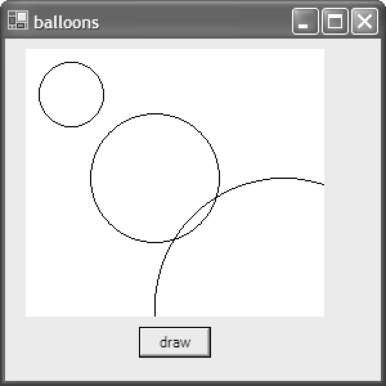
\includegraphics[width=7cm]{data_balloons_screen}
			\caption{Display of balloons.}
			\label{fig:data_balloons_screen}
		\end{figure}
		\begin{lstlisting}
Private Sub DisplayBalloons()
	Dim myPen As Pen = New Pen(Color.Black)
	Dim drawArea As Graphics
	drawArea = PictureBox1.CreateGraphics()
	drawArea.Clear(Color.White)
	For Each b As Balloon In party
		b.Display(drawArea, myPen)
	Next
End Sub
		\end{lstlisting}

	\section{Programming principles}
		List boxes are perhaps the simplest kind of data structure provided by Visual Basic. They enable a list of strings to be assembled, displayed and manipulated. A data structure is a group of data items that can be processed in a uniform manner. Because they can be made visible, list boxes are a good way of learning about data structures.

		A list box employs a list object to store the information. Like a list box, a list expands and contracts as necessary. A data structure such as a list is set up in the main memory of the computer (not on backing storage) so that it exists only as long as the program runs. When the program terminates, the data structure is destroyed.

		Lists are one of the classic structures in computing. One of the oldest and most venerated languages, LISP (short for List Processing), uses nothing but lists. A list is a sequence of items that can grow and shrink in length. Items can be added to the end of a list and removed from anywhere within the list. Also the values of items within a list can be changed. Thus a list is a flexible structure for representing a collection of items that are related in some way. Most types of data structure are invisible and, if required, a list box can be made invisible.

		Another major type of data structure is the array (explained in \Cref{ch:arrays}). An array is a collection of similar data items, each distinguished by an index. Unlike a list box, an array is invisible and when items need to be displayed, the programmer must write explicit instructions to do it. Furthermore, although items can be inserted and removed from the body of a list box, arrays do not support these facilities.
		
		In circumstances where all the items in a list box need processing, the natural control structure is a \keyword{For} loop.
		
		The task of finding the largest item in a list of numbers is a classic problem in programming. This is also true of the search method.


	\section{Programming pitfalls}
		A common error is to think that index values start at 1. (They start at 0.)

	\section{New language elements}
		\keyword{For Each} provides a convenient and concise way of looping through all the values of a data structure such as a list.
	
		The generics facility allows us to specify the class of objects that a list will contain. This is done using the keyword Of. For example:
		\begin{lstlisting}
Private party As New List(Of Balloon)
		\end{lstlisting}

	\section{Summary}
		\begin{itemize}
      \item A list box is a GUI box that contains a list of strings.
      \item Each item in a list box is uniquely identified by an integer, called an index. Index values are not stored. Index values always start at 0.
      \item A program can add items to the end of a list box, remove an item, change an item or insert an item anywhere within a list box.
			\item A list box employs a list (\keyword{List}) object to store the information in the list. It is the list object that supports the methods to add and remove items from a list box.
      \item A list holds a collection of data values or objects. Such a list grows or shrinks according to how much data it contains.
      \item Each item in a list is uniquely identified by an integer, an index.
      \item When a list is created, the programmer states what kind of objects it will contain.
			\item A set of methods is provided to act on a list. They include \keyword{Add}, \keyword{Clear}, \keyword{Contains}, \keyword{IndexOf}, \keyword{Insert}, \keyword{RemoveAt}, \keyword{Remove}.
      \item Generics allow the programmer to specify the type of items that a list holds.
		\end{itemize}

	\section{Exercises}
		\begin{EXE}
			\item	Write a program in which an item selected in a list box (by clicking on it) is immediately deleted. Alternatively, provide a 'delete' button to delete the item that is currently selected.
			\item Alter the program so that items in the list box are automatically always sorted into alphabetical order. (To accomplish this, investigate the properties of list box.)
			\item Add a button that causes the list box to be emptied, using the method Clear.
			\item Alter the program so that an item in the list box can be replaced by some other text. For example, 'milk' is replaced by 'sugar'. Provide a button marked 'replace' that carries out this action. The new text is to be entered into a text box.
			\item Write a program that allows items to be inserted or removed from any position within a list box, using suitable buttons.
			\item Improve the search method so that it displays a message whether or not the required item is found in the list box.
		\end{EXE}

		\begin{stab}
			\begin{enumChapter}
				\item	0
				\item milk
				\item Change the greater-than sign to a less-than sign.
			\end{enumChapter}
		\end{stab}
